\begin{figure}[H]
        \centering 
        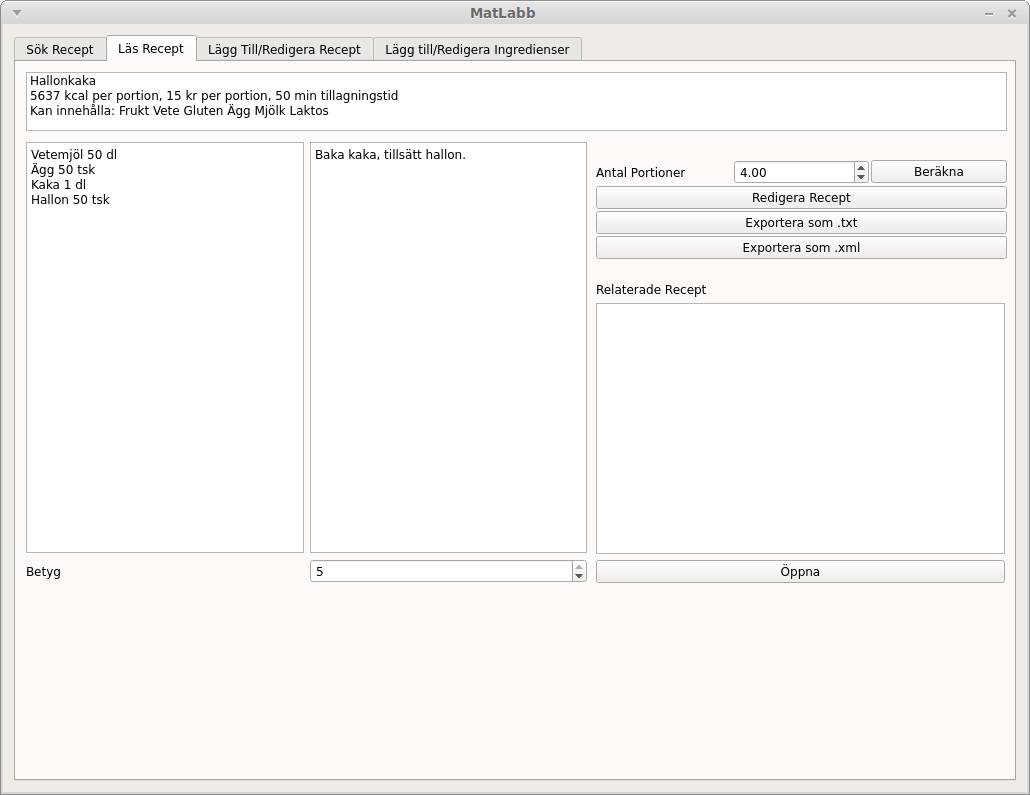
\includegraphics[scale=0.44]{las_recept.png} 
        \caption{Läs receptvyn} 
        \label{fig:receptvyn}
\end{figure}

I \verb+Läs recept+-vyn möts man av en rad fält. I huvudfältet längst upp finner
man information om receptets namn antal kilokalorier per portion,
antal kronor per portion och hur lång tid receptet tar att laga.

Under huvudfönstret finns från vänster sett Ingrediensfältet,
instruktionsfältet samt kommentarsfältet. I ingrediensfältet finns de
ingredienser som krävs samt åtgångsmängd, i instruktionsfältet finns
instruktioner och i kommentarsfältet finns det möjlighet för korta
kommentarer ifall man inte önskar att ändra receptet.
